%-----------------------------------------------------------------------------
% APPLICATION
%-----------------------------------------------------------------------------
\section{Application: Sales Agent}
\label{sec:application}

\subsection{System Overview}
\label{subsec:overview}

The Sales Agent is an LLM-powered conversational system designed to enable business analysts
to query and explore retail sales data using natural language, without requiring knowledge of SQL
or any underlying data infrastructure. Given a question expressed in plain English, the agent
autonomously determines the appropriate processing steps, retrieves the relevant data, produces
a textual analysis, and optionally generates a chart to support data-driven decision making.

The system operates on a synthetic retail dataset composed of three relational tables stored in
Parquet format: \textit{sales}, which records daily store-level transactions with pricing and
promotion information; \textit{products}, which contains the product catalog including category,
brand, unit price, and origin; and \textit{stores}, which holds store metadata such as location,
type, size, and staffing. The tables are linked through shared keys (\texttt{Store\_Number} and
\texttt{SKU\_Coded}), allowing the agent to answer questions that span multiple entities through
SQL JOIN operations.

The agent is orchestrated via LangGraph~\cite{langgraph}, a framework for building stateful,
graph-based LLM pipelines. At each invocation, the user's natural language question is routed
through a directed graph of processing nodes: a \textit{tool selection} node decides which tools
to activate, a \textit{lookup} node generates and executes a SQL query via DuckDB to retrieve
structured data, an \textit{analysis} node produces a natural language summary of the results,
and a \textit{visualization} node generates Python chart code. The LLM backbone is configurable:
the system supports both locally-hosted models via Ollama and cloud-based models via the OpenAI API,
making it suitable for deployment in both resource-constrained and high-performance environments.

Figure~\ref{fig:system_overview} illustrates the high-level architecture of the Sales Agent,
showing the flow from user input to final output across the agent's processing pipeline.

\begin{figure}[h]
    \centering
    \vspace{-8pt}
    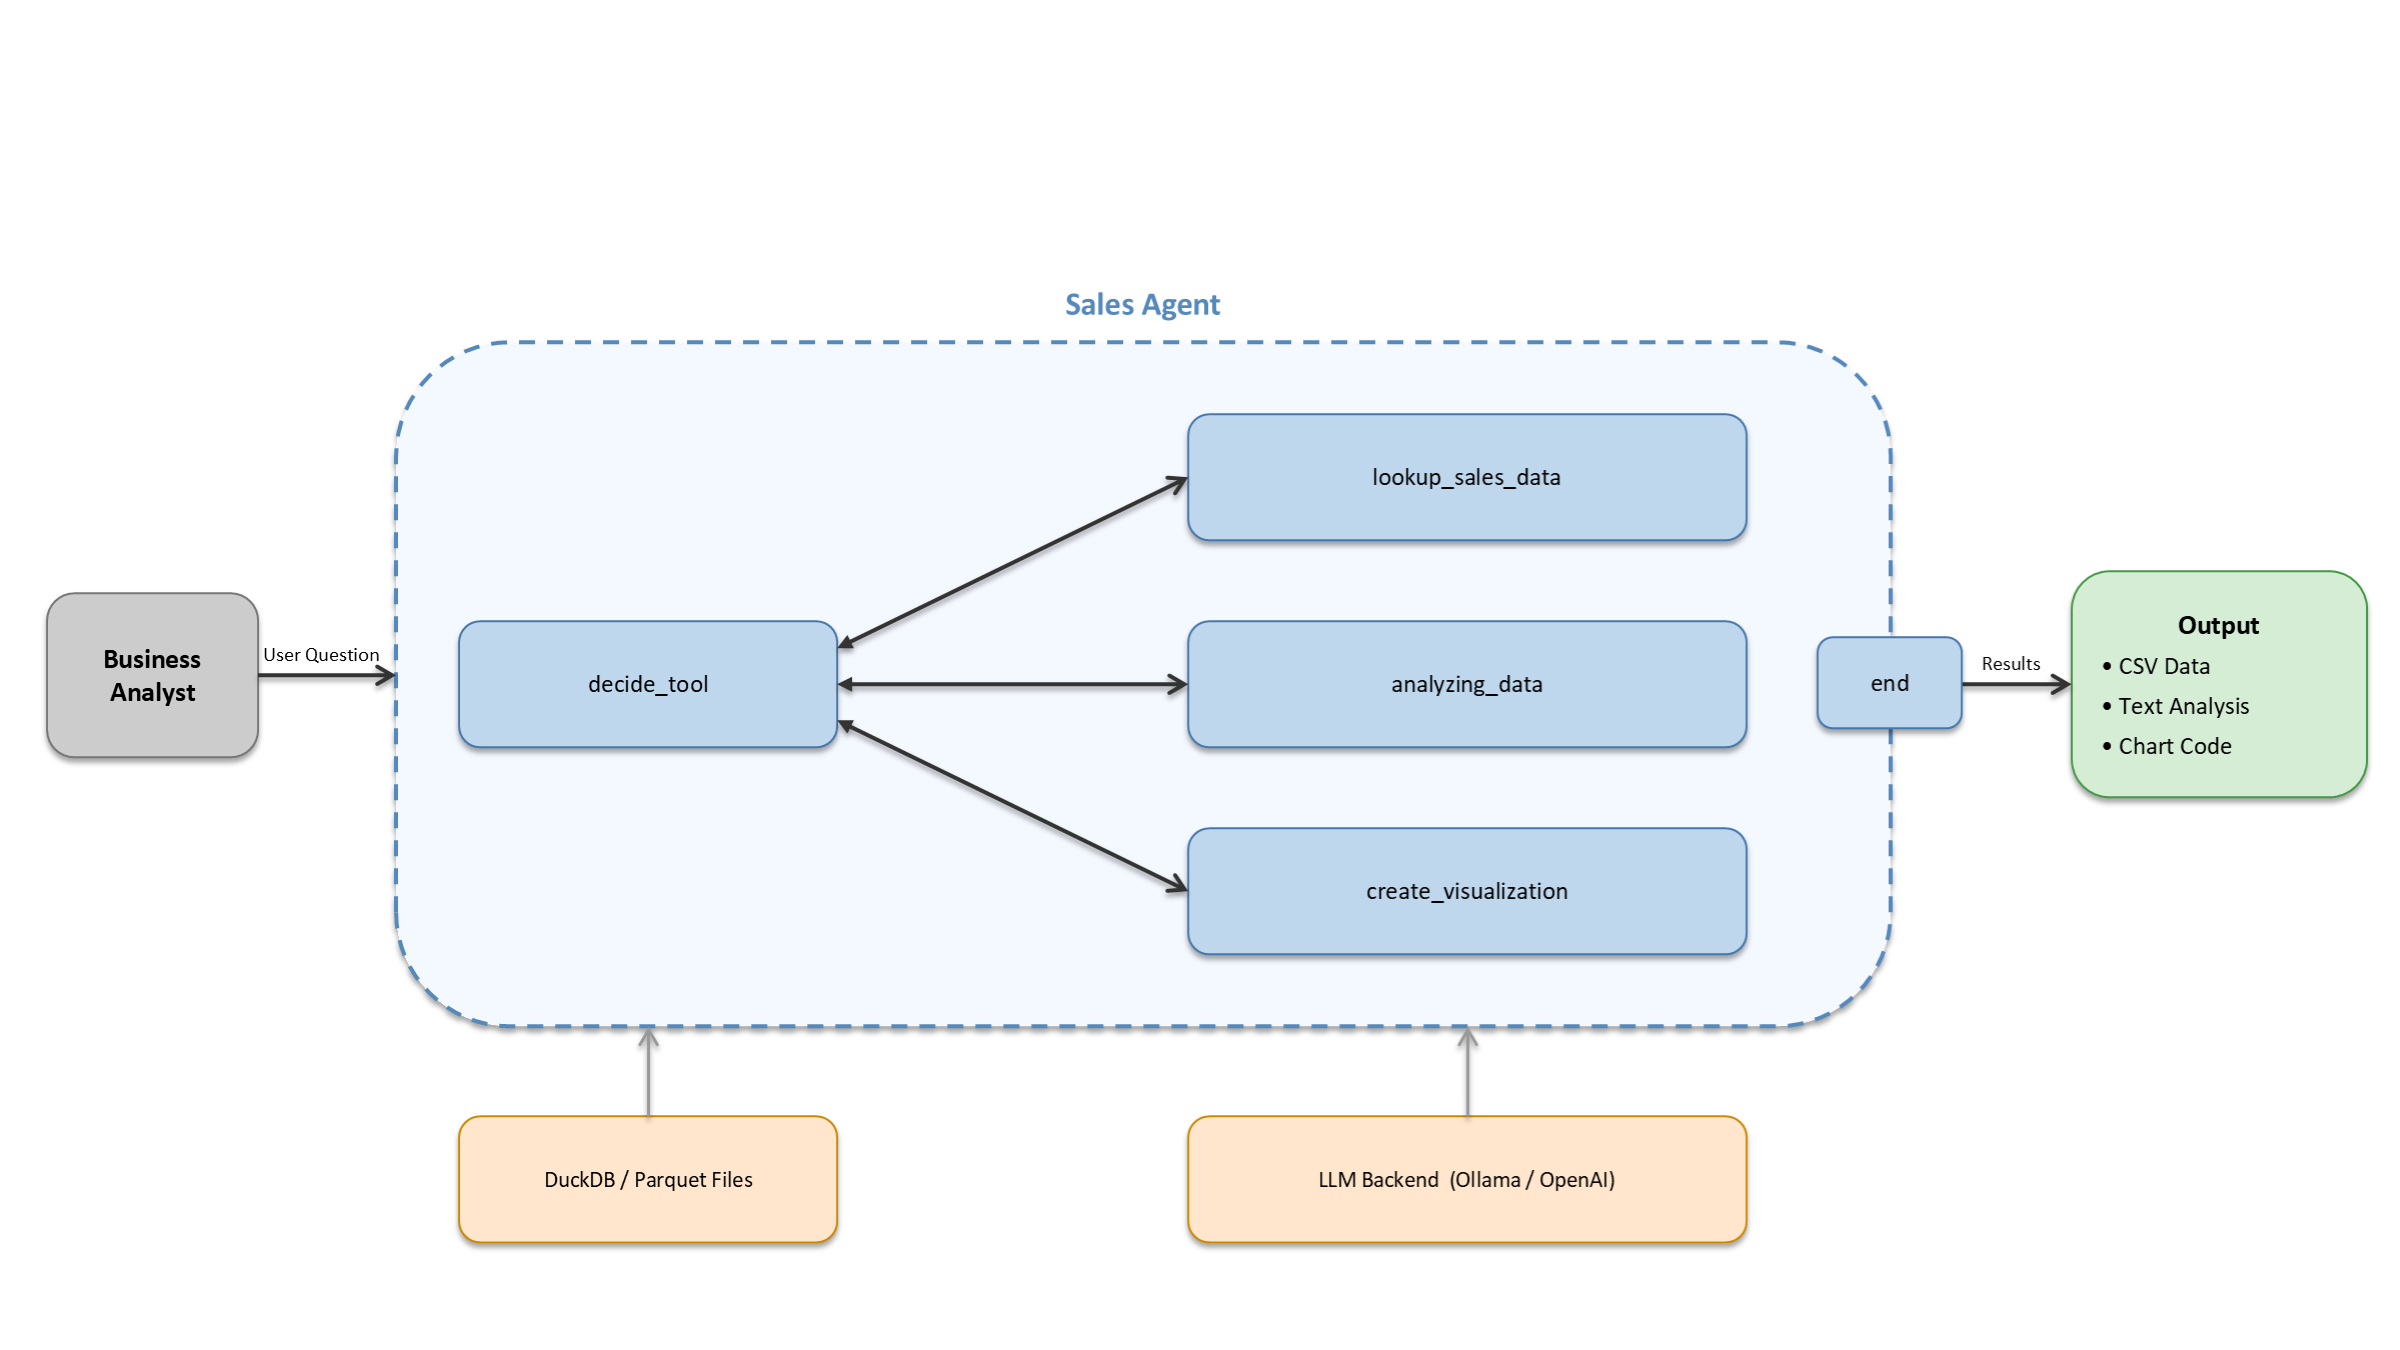
\includegraphics[width=0.92\textwidth]{Images/fig1_system_overview}
    \caption{High-level architecture of the Sales Agent.}
    \label{fig:system_overview}
\end{figure}

The output of the system consists of three complementary components: a structured CSV table
containing the query results, a natural language analysis interpreting the data in the context
of the original question, and an executable Python script that renders a visualization of the
findings. This multi-modal output is designed to cover the full analytical workflow of a business
analyst, from raw data retrieval to presentation-ready charts.

\subsection{System Architecture}
\label{subsec:architecture}

The Sales Agent is implemented as a Python package organised into six modules,
each with a clearly delimited responsibility. Figure~\ref{fig:class_diagram} shows
the class diagram of the system.

\begin{figure}[h]
    \centering
    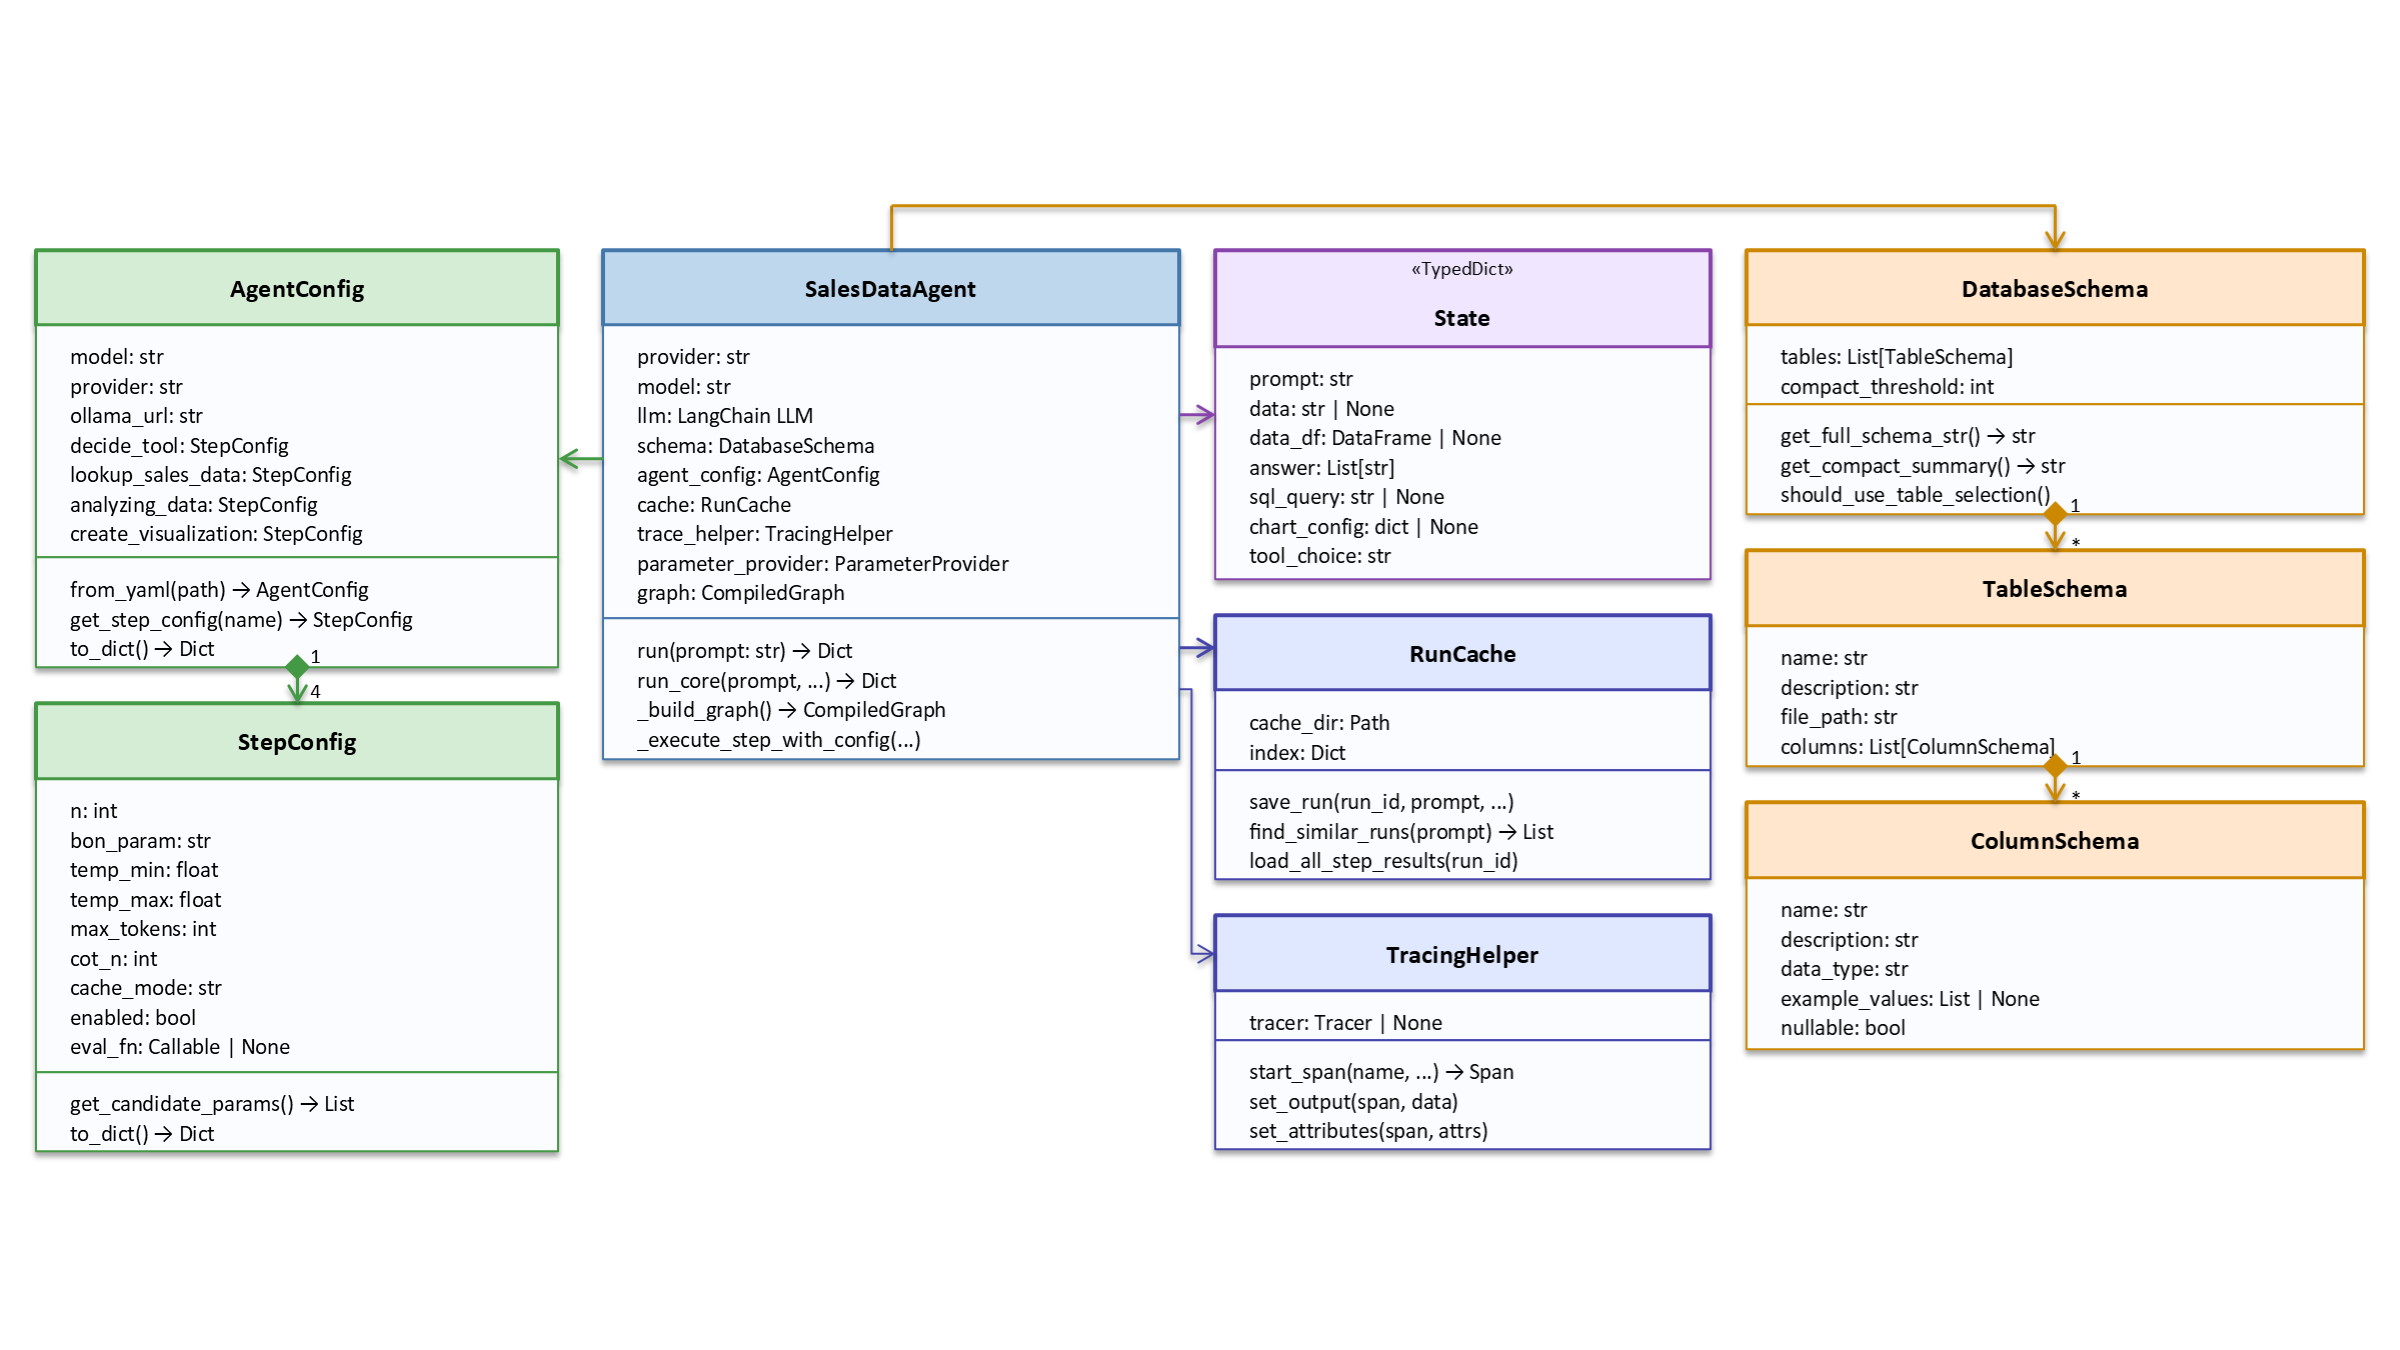
\includegraphics[width=0.98\textwidth]{Images/fig2_class_diagram.png}
    \vspace{-10pt}
    \caption{Class diagram of the Sales Agent.}
    \label{fig:class_diagram}
\end{figure}

\textbf{SalesDataAgent} is the main entry point of the system. It builds the LangGraph
execution graph, wires the processing nodes together, and exposes a single \texttt{run()}
method that accepts a natural language prompt and returns the final result dictionary.
It holds references to the \texttt{AgentConfig}, the \texttt{DatabaseSchema}, and the
\texttt{RunCache}, and coordinates the end-to-end execution including tracing and
energy monitoring.

\textbf{AgentConfig} and \textbf{StepConfig} form the configuration layer.
\texttt{AgentConfig} holds global settings — the LLM provider (\texttt{ollama} or
\texttt{openai}), the model name, and the Ollama server URL — together with one
\texttt{StepConfig} instance per processing step. \texttt{StepConfig} encapsulates
all per-step hyperparameters: number of best-of-$n$ candidates, temperature range,
top-$p$, top-$k$, beam width, maximum tokens, caching policy, and optional evaluation
and selection callables. Both classes support serialisation to and from dictionaries
and YAML files, enabling fully reproducible experiment configurations.

\textbf{State} is a \texttt{TypedDict} that acts as the shared memory flowing through
the LangGraph nodes. It carries the user prompt, the retrieved data (as both a CSV
string and a Pandas \texttt{DataFrame}), the generated SQL query, the chart
configuration, the tool choice, per-step timing and evaluation scores, and the
ground-truth scores accumulated during benchmarking.

\textbf{DatabaseSchema}, \textbf{TableSchema}, and \textbf{ColumnSchema} define the
multi-table data model exposed to the LLM. \texttt{DatabaseSchema} wraps a list of
\texttt{TableSchema} objects and provides two rendering modes: a compact summary
(table names and descriptions only) used when the number of tables exceeds a
configurable threshold, and a full schema string including all column names, types,
descriptions, and example values used during SQL generation.

\textbf{RunCache} manages persistent caching of agent runs on disk. Each completed
run is stored under a unique \texttt{run\_id} directory containing the per-step
results for all $n$ best-of-$n$ candidates. A JSON index file enables fast lookup
of lexically similar past runs by prompt word overlap (Jaccard similarity over the
prompt token sets), allowing the agent to reuse previously computed results and
avoid redundant LLM calls.

\textbf{TracingHelper} provides optional observability integration via
OpenTelemetry~\cite{opentelemetry} and the Arize Phoenix platform~\cite{arize_phoenix}. When enabled,
it records structured spans for each processing step, capturing inputs, outputs,
latencies, and evaluation scores for post-hoc analysis.

\vspace{0.5em}
\noindent The system depends on the following key external libraries:

\begin{itemize}
    \item \textbf{LangGraph} / \textbf{LangChain} — graph-based LLM pipeline
          orchestration and provider-agnostic LLM interfaces (OpenAI, Ollama);
    \item \textbf{DuckDB} — in-process analytical SQL engine used to query Parquet files;
    \item \textbf{Pandas} / \textbf{PyArrow} — tabular data manipulation and Parquet I/O;
    \item \textbf{Matplotlib} — chart rendering for the visualisation step;
    \item \textbf{CodeCarbon} — energy consumption tracking during agent execution;
    \item \textbf{NLTK} — natural language utilities available for optional
          n-gram-based text scoring (e.g.\ BLEU), not used by the LLM-as-judge
          metrics adopted in the experiments;
    \item \textbf{PyYAML} — parsing of experiment configuration files;
\end{itemize}

\subsection{LangGraph Workflow}
\label{subsec:langgraph}

The execution logic of the Sales Agent is modelled as a directed cyclic graph built
with LangGraph's \texttt{StateGraph} API. The graph has four processing nodes and a
single terminal node (\texttt{END}), as illustrated in Figure~\ref{fig:langgraph}.

\begin{figure}[h]
    \centering
    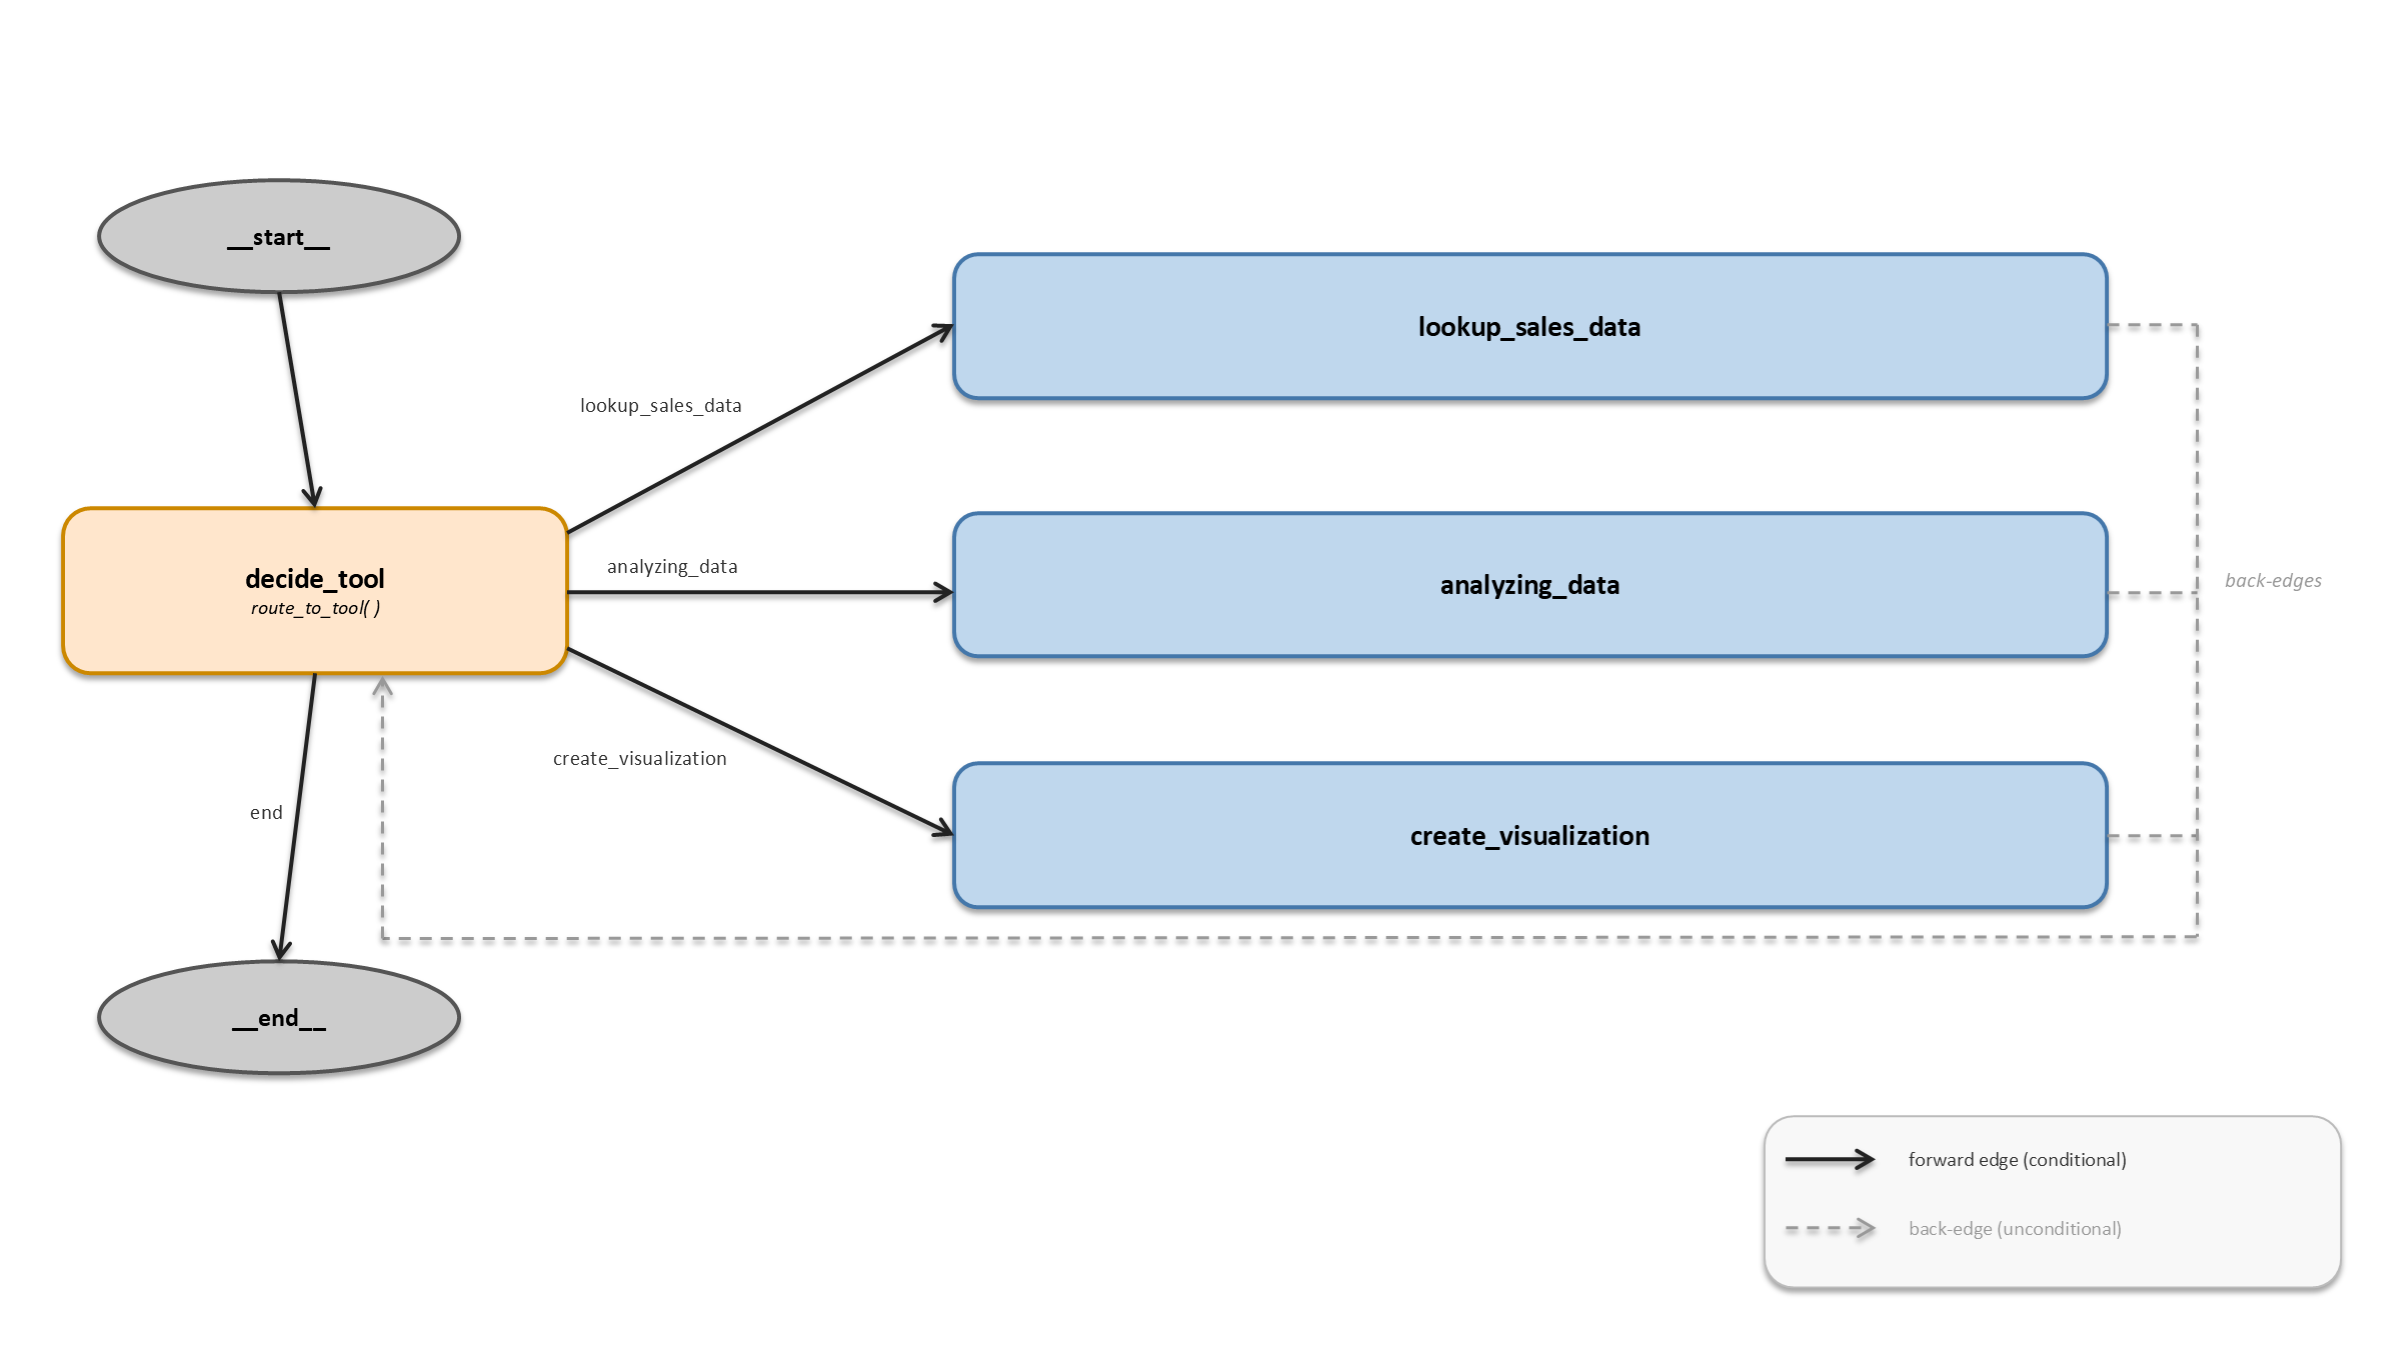
\includegraphics[width=0.85\textwidth]{Images/fig3_langgraph.png}
    \vspace{-10pt}
    \caption{LangGraph execution graph of the Sales Agent.}
    \label{fig:langgraph}
\end{figure}

\noindent The graph is defined as follows:

\begin{itemize}
    \item \textbf{Entry point}: \texttt{decide\_tool} — every execution starts here.
    \item \textbf{Conditional edges from \texttt{decide\_tool}}: the routing function
          \texttt{route\_to\_tool} reads the \texttt{tool\_choice} field set by the node
          and dispatches to one of \texttt{lookup\_sales\_data}, \texttt{analyzing\_data},
          \texttt{create\_visualization}, or \texttt{END}.
    \item \textbf{Back-edges}: after each processing node completes, an unconditional
          edge returns control to \texttt{decide\_tool}, forming a loop that continues
          until the LLM decides to terminate.
\end{itemize}

\paragraph{The \texttt{decide\_tool} node.}
At each iteration, this node invokes the LLM with a structured prompt describing the
four available tools, the current state of the conversation (user question, answers
generated so far, last tool used), and a Chain-of-Thought reasoning template.
The LLM reasons through five steps — analysing the user request, checking progress,
identifying what is missing, verifying decision rules, and making the final choice —
and outputs a single tool name. The routing is governed by three hard rules:
(1)~\texttt{lookup\_sales\_data} must run before any analysis or visualisation;
(2)~no tool may be selected more than once per execution;
(3)~\texttt{end} is selected when at least two answers have been generated or all
relevant tools have been executed.
Fuzzy string matching is applied to the raw LLM output to tolerate minor formatting
variations.

\paragraph{The \texttt{lookup\_sales\_data} node.}
This node generates a SQL query from the user prompt and the database schema, executes
it against the Parquet files via DuckDB, and stores the result in the \texttt{State}
as both a CSV string and a Pandas \texttt{DataFrame}.
When best-of-$n$ sampling is enabled (\texttt{StepConfig.n} $> 1$), the node generates
$n$ candidate SQL queries at different temperature values and selects the one with the
highest evaluation score before writing the result to the state.

\paragraph{The \texttt{analyzing\_data} node.}
Given the retrieved data and the original question, this node prompts the LLM to produce
a natural language analysis. The generated text is appended to the \texttt{answer} list
in the \texttt{State}.

\paragraph{The \texttt{create\_visualization} node.}
This node first asks the LLM to produce a structured chart configuration (chart type,
axes, title, colour scheme), then generates executable Python code using Matplotlib
that renders the chart from the retrieved data. Both the configuration and the code
are stored in the \texttt{State} and appended to the \texttt{answer} list.

\vspace{0.5em}
Figure~\ref{fig:sequence} shows the sequence diagram for a full execution of the
Sales Agent on a question that requires data retrieval, analysis, and visualisation.
The notation follows a deliberately simplified variant of UML~2 sequence diagrams:
standard lifelines and message arrows are retained, combined fragments (\texttt{loop}
and \texttt{opt}) mark the iteration boundary and the optional table-selection step,
and dashed arrows denote return values. Activation bars, actor stereotypes (e.g.\
stick figures or boundary symbols), and explicit \emph{create}/\emph{destroy} messages
have been omitted. Given the density of the diagram~--- nine lifelines and approximately
35 messages across four iterations~--- these elements would add visual noise without
improving comprehension; the colour coding of the participant boxes already conveys
their roles at a glance. This choice prioritises readability over strict UML compliance,
which is standard practice in academic and industrial documentation when the primary
goal is to communicate flow rather than to specify a system for code generation.

\begin{figure}[htbp]
    \centering
    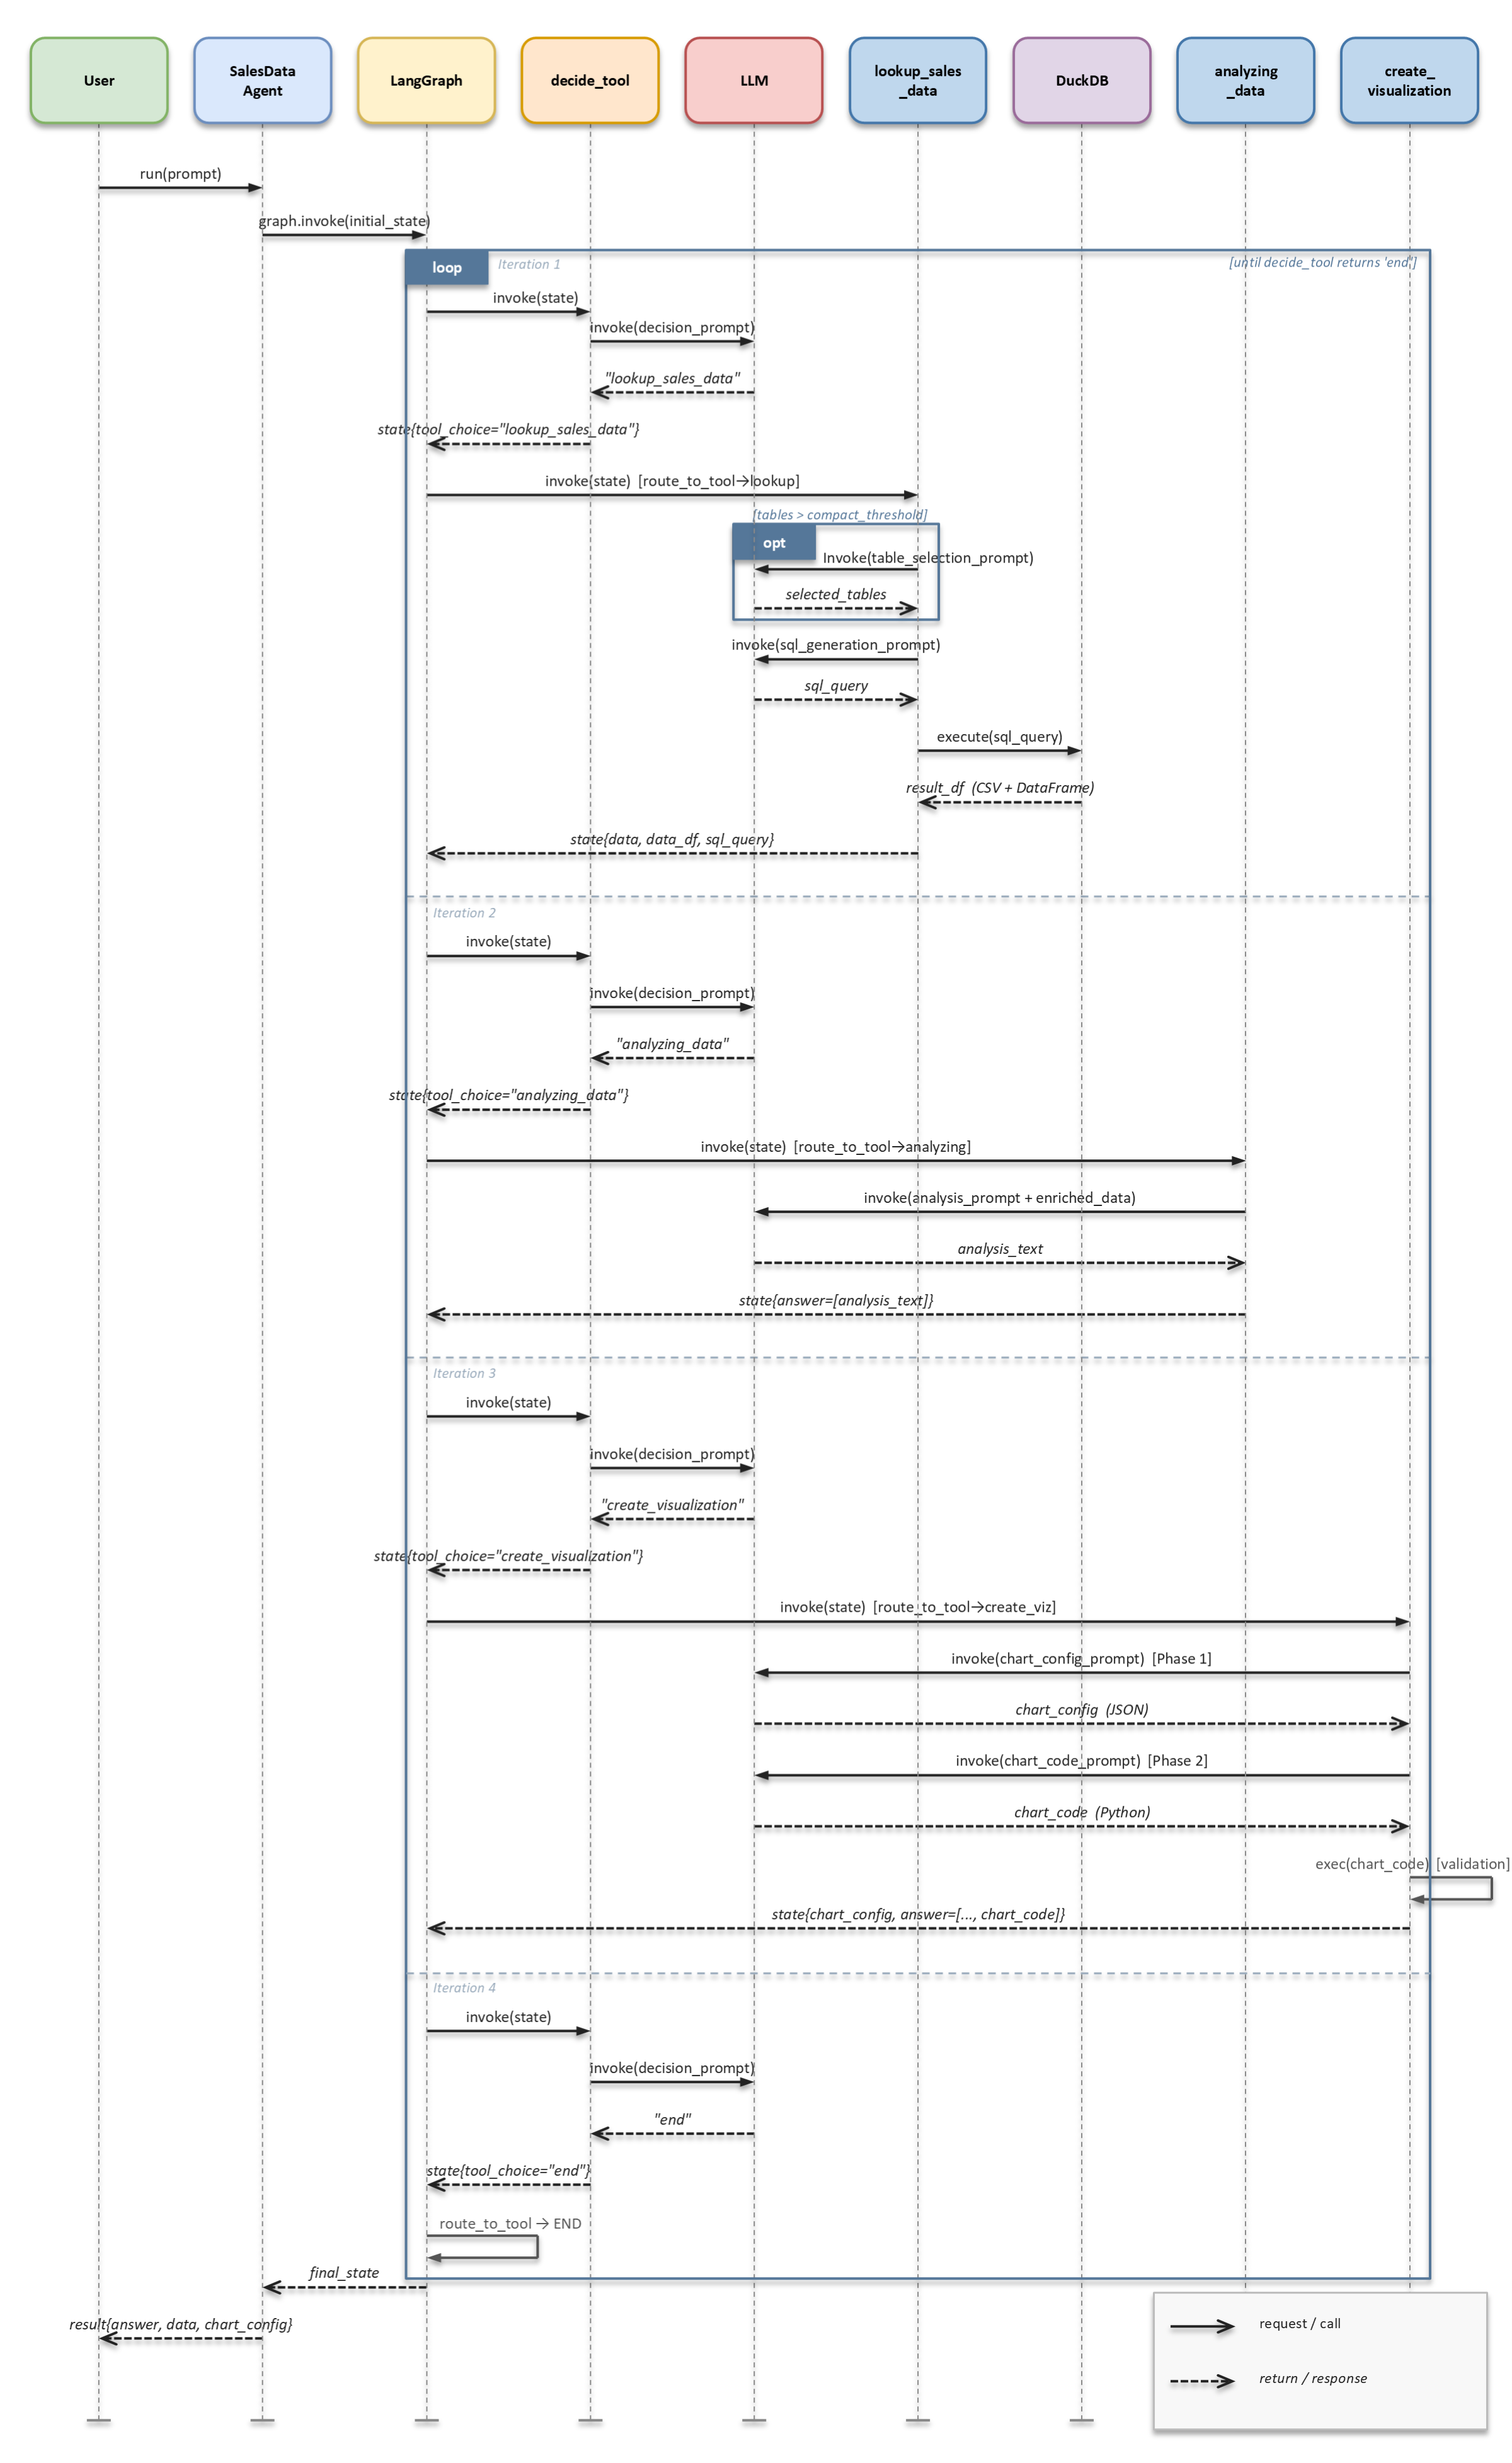
\includegraphics[width=0.65\textwidth]{Images/fig4_sequence.png}
    \vspace{-6pt}
    \caption{Sequence diagram of a full Sales Agent execution.}
    \label{fig:sequence}
\end{figure}

The system also supports two restricted operating modes configured via the
\texttt{agent\_mode} parameter in the YAML file: \texttt{lookup\_only} skips both
analysis and visualisation, returning only the raw query result; \texttt{analysis}
skips visualisation and returns data plus text analysis. These modes reduce latency
and LLM cost when the full output is not required.

\subsection{Agent Tools and Steps}
\label{subsec:tools}

Each of the three processing nodes of the Sales Agent encapsulates a distinct
analytical capability. This section describes their internal logic in detail.

\subsubsection{Lookup Tool}

The \texttt{lookup\_sales\_data} step is responsible for translating the user's
natural language question into a SQL query and executing it against the Parquet
dataset via DuckDB.

The step opens a fresh in-process DuckDB connection for each invocation and
registers all Parquet files as named SQL tables. It then builds the schema context
— either the full column-level description or, when the number of tables exceeds
\texttt{compact\_threshold}, the output of the two-step table selection procedure
described in Section~\ref{subsec:multitable}. The LLM receives the schema context
together with the user prompt and a Chain-of-Thought SQL generation prompt, and
produces a SQL query. The query is executed via \texttt{duckdb.execute()}, and the
result is stored in the \texttt{State} as both a CSV string (\texttt{data}) and a
Pandas \texttt{DataFrame} (\texttt{data\_df}).

Before passing the retrieved data to the analysis step, the system enriches it with
pre-computed aggregate statistics: for every numeric column, the sum, minimum,
maximum, and mean are appended to the CSV string as a dedicated summary block.
This prevents the LLM from having to perform arithmetic over potentially hundreds of
rows, improving both accuracy and consistency of the generated analysis.

\subsubsection{Analysis Tool}

The \texttt{analyzing\_data} step takes the enriched CSV data and the original user
prompt and asks the LLM to produce a concise natural language interpretation of the
results. The prompt instructs the model to answer using only the values present in
the data, to cite specific numbers, and to avoid speculation. A Chain-of-Thought
template guides the model through understanding the question, examining the data,
identifying key insights, and formulating a clear answer. The generated text is
appended to the \texttt{answer} list in the \texttt{State}.

\subsubsection{Visualization Tool}

The \texttt{create\_visualization} step is a two-phase process. In the first phase,
the LLM is asked to extract a structured chart configuration from the data and the
user's question: it outputs a JSON-like dictionary specifying the chart type (bar,
line, scatter, etc.), the columns to use for the $x$ and $y$ axes, the chart title,
and any grouping or colour dimensions. In the second phase, a second LLM call
receives the chart configuration and the \texttt{DataFrame} and generates executable
Python code using Matplotlib that renders the requested chart.

Once generated, the code is immediately validated by executing it in an isolated
namespace using Python's built-in \texttt{exec()} function. The Matplotlib backend
is switched to \texttt{Agg} (non-interactive, headless) prior to execution to avoid
graphical environment dependencies. If the code raises an exception, the error
message is stored in the \texttt{State} and can be fed back to the LLM by the CoT
refinement mechanism (described in Section~\ref{subsec:prompting}) for iterative
correction. The validated code and the chart configuration are both appended to the
\texttt{answer} list.

\subsection{LLM Integration and Prompting Techniques}
\label{subsec:prompting}

\subsubsection{Supported LLM Backends}

The Sales Agent is designed to be provider-agnostic. Two backends are supported and
can be selected via the \texttt{provider} field in \texttt{AgentConfig}:

\begin{itemize}
    \item \textbf{OpenAI} — cloud-based models accessed through the OpenAI API
          (e.g.\ \texttt{gpt-4o-mini}, \texttt{gpt-4o}). Authentication is handled
          via an API key passed through the configuration file or environment variable.
    \item \textbf{Ollama} — locally-hosted open-weight models served via the Ollama
          runtime (e.g.\ \texttt{llama3.2:3b}, \texttt{qwen2.5:7b}). The server URL
          is configurable, enabling deployment on remote GPU machines.
\end{itemize}

Both backends are accessed through the LangChain abstraction layer
(\texttt{langchain-openai} and \texttt{langchain-ollama}), so the step functions
are completely agnostic to the underlying provider. Per-step provider and model
overrides are also supported: it is possible, for example, to use a large cloud
model for SQL generation and a smaller local model for routing.

\subsubsection{Prompt Structure}

All prompts in the Sales Agent share a common skeleton. Each prompt opens with a
\textbf{role declaration} that assigns a persona to the model (e.g.\
\textit{``You are an expert SQL developer specialising in DuckDB queries''}), followed
by a \textbf{Markdown-sectioned body} that separates concerns into labeled blocks:
\texttt{\#\# TASK} (what to produce), \texttt{\#\# AVAILABLE DATA} / \texttt{\#\# USER QUESTION}
(dynamic context injected via template variables at runtime), \texttt{\#\# INSTRUCTIONS}
(generation rules), and \texttt{\#\# OUTPUT FORMAT} (exact specification of what the
model should return). Keeping the static scaffold and the dynamic content clearly
separated simplifies both prompt maintenance and output parsing.

\subsubsection{Chain-of-Thought Prompting}

Three of the four agent prompts — tool routing, data analysis, and chart configuration
— augment the shared structure above with a \texttt{\#\# CHAIN OF THOUGHT REASONING}
section~\cite{wei2022chain}. This section defines a sequence of named steps (e.g.\
\textit{Step 1: Understanding the Question}, \textit{Step 2: Examining the Data
Structure}, \ldots) that the model must work through and expose in its output before
producing the final answer. By externalising intermediate reasoning, the model is less
likely to skip steps or make implicit assumptions, and the output is easier to inspect
and validate.

The SQL generation prompt deliberately omits the CoT reasoning section.
During development, smaller open-weight models tended to lose track
of critical constraints — DuckDB-specific syntax rules, column qualification in JOINs,
and the required plain-text output format — when required to produce explicit
step-by-step reasoning before the query. The additional text generation appeared to
exhaust the model's effective attention on the earlier instruction blocks. The SQL
prompt therefore replaces the CoT section with a \texttt{\#\# COMMON MISTAKES TO AVOID}
block listing wrong/right DuckDB patterns, and a \texttt{\#\# EXAMPLES} block of
few-shot query pairs, while the \texttt{\#\# OUTPUT FORMAT} section explicitly
instructs the model to return only the plain SQL with no explanations or markdown.
This change consistently reduced syntax errors and instruction-following failures
across the small models tested.

\subsubsection{Best-of-\texorpdfstring{$N$}{N} Sampling}

For steps where output quality is critical — SQL generation and data analysis in
particular — the agent supports best-of-$N$ sampling. When \texttt{StepConfig.n}
$> 1$, the step is executed $N$ times with different values of the sampling parameter
specified by \texttt{bon\_param} (temperature, top-$p$, or top-$k$), linearly
interpolated between \texttt{temp\_min} and \texttt{temp\_max} (or the corresponding
bounds for top-$p$ and top-$k$). Each of the $N$ candidate outputs is independently
scored by the \texttt{eval\_fn} assigned to that step, and the candidate with the
highest score is selected via \texttt{selection\_fn} (defaulting to argmax). All $N$
results are saved to the \texttt{RunCache} to allow re-selection with different
evaluation criteria without re-invoking the LLM.

\subsubsection{Iterative CoT Refinement}

For steps with \texttt{StepConfig.cot\_n} $> 1$, the agent applies iterative
Chain-of-Thought refinement. After the initial LLM call, the output is fed back into
the same prompt through a \texttt{CoTRefinementLLM} wrapper. This wrapper appends a
refinement block to every subsequent call, showing the model its previous response
and asking it to either confirm it (if correct and complete) or produce an improved
version. The loop runs for at most \texttt{cot\_n} total iterations, but stops early
as soon as the output converges — i.e.\ when the textual similarity between two
consecutive responses reaches or exceeds 0.95 — avoiding redundant refinement calls
once the model has settled on a stable answer.

Two refinement modes are available. In the standard mode, the model receives its
previous output and can voluntarily refine it. In error-aware mode, triggered when
the visualization code raises an exception during validation, the error message is
explicitly included in the refinement block with a directive to fix it. This
self-correction loop allows the agent to recover from syntactically or semantically
incorrect code without user intervention.

\subsection{Configuration System}
\label{subsec:config}

The Sales Agent exposes a hierarchical configuration system that controls every
aspect of the agent's behaviour without requiring code changes. All settings are
defined in a single YAML file and loaded at startup via \texttt{AgentConfig.from\_yaml()}.

\subsubsection{YAML Structure}

The configuration file is divided into six top-level sections:

\begin{itemize}
    \item \texttt{agent} — global LLM settings: provider (\texttt{openai} or
          \texttt{ollama}), model name, Ollama server URL, and OpenAI API key;
    \item \texttt{steps} — per-step hyperparameters, one sub-section per node
          (\texttt{decide\_tool}, \texttt{lookup\_sales\_data}, \texttt{analyzing\_data},
          \texttt{create\_visualization});
    \item \texttt{schema} — path to the data directory containing the
          \texttt{*\_schema.yaml} files and the \texttt{compact\_threshold} value;
    \item \texttt{run} — execution parameters: prompt, visualisation goal, operating
          mode, run identifier, output directory, caching options, and CodeCarbon flag;
    \item \texttt{ground\_truth} — optional ground-truth references for tracking
          evaluation scores during benchmarking (described in
          Section~\ref{subsec:benchmark});
    \item \texttt{tracing} — optional Phoenix/OpenTelemetry endpoint for observability.
\end{itemize}

\subsubsection{Per-Step Parameters}

Each step exposes the parameters listed in Table~\ref{tab:stepconfig}. A step can
also override the global LLM provider and model, enabling heterogeneous deployments
where, for example, SQL generation uses a larger cloud model while routing uses a
lightweight local model.
The default values shown reflect the baseline configurations used in the experiments
(Section~\ref{sec:experimentdesign}): Gemma~4 models are run at temperature~1.0, which
is the recommended setting for thinking models; Mistral~Small~3.2 is run at
temperature~0.15, appropriate for an instruction-following model.

\begin{table}[H]
\centering
\begin{tabular}{|l|l|l|p{4.5cm}|}
\arrayrulecolor{black}\hline
\rowcolor{bluePoli!30}
\textbf{Parameter} & \textbf{Default (Gemma~4)} & \textbf{Default (Mistral)} & \textbf{Description} \T\B \\
\arrayrulecolor{black}\hline
\texttt{n} & 1 & 1 & Number of best-of-$n$ candidates \T\B \\
\hline
\texttt{bon\_param} & \texttt{temperature} & \texttt{temperature} & Parameter varied across candidates \T\B \\
\hline
\texttt{temp\_min / temp\_max} & 1.0 / 1.0 & 0.15 / 0.15 & Temperature range for sampling \T\B \\
\hline
\texttt{top\_p\_min / top\_p\_max} & 0.95 / 0.95 & 0.95 / 0.95 & Top-$p$ nucleus sampling range \T\B \\
\hline
\texttt{top\_k\_min / top\_k\_max} & 64 / 64 & 64 / 64 & Top-$k$ sampling range (Ollama only) \T\B \\
\hline
\texttt{num\_beams} & 1 & 1 & Beam search width; 1 = greedy (Ollama only) \T\B \\
\hline
\texttt{repeat\_penalty} & 1.1 & 1.1 & Repetition penalty applied to already-seen tokens; $>1$ discourages repetition (Ollama only) \T\B \\
\hline
\texttt{repeat\_last\_n} & 64 & 64 & Lookback window (tokens) over which the repetition penalty is applied; 0 disables it (Ollama only) \T\B \\
\hline
\texttt{max\_tokens} & 5000 / 7000 & 5000 / 7000 & Maximum tokens per LLM generation (5000 for lookup, 7000 for analysis and visualization) \T\B \\
\hline
\texttt{cot\_n} & 1 & 1 & Maximum CoT refinement iterations \T\B \\
\hline
\end{tabular}
\caption{Configurable parameters of \texttt{StepConfig}.}
\label{tab:stepconfig}
\end{table}

\subsubsection{Runtime Overrides}

The \texttt{run.step\_overrides} field allows temporary parameter changes for a
single execution without modifying the base configuration. For example, setting
\texttt{analyzing\_data.n: 3} and \texttt{temp\_max: 1.3} increases best-of-$n$
sampling for the analysis step in that run only. Runtime overrides are mediated by
a pluggable \texttt{ParameterProvider} abstraction, queried before each step to
return the effective \texttt{StepConfig}: the default \texttt{DefaultProvider}
returns the static YAML configuration unchanged, while the \texttt{interactive\_config}
flag activates a \texttt{TerminalProvider} that prompts the user to accept or
override the step parameters at runtime (falling back to the defaults when no
interactive terminal is available), useful for exploratory experiments.

\subsection{Multi-Table Support and Dataset}
\label{subsec:multitable}

\subsubsection{Dataset Description}

The Sales Agent operates on a synthetic retail dataset composed of three relational
tables stored as Parquet files. The dataset was generated programmatically to
simulate a realistic grocery retail scenario spanning multiple stores, product
categories, and time periods. Table~\ref{tab:dataset} summarises the three tables
and their key columns.

\begin{table}[H]
\centering
\arrayrulecolor{black}
\begin{tabular}{|l|p{5.5cm}|p{5cm}|}
\hline
\rowcolor{bluePoli!30}
\textbf{Table} & \textbf{Key columns} & \textbf{Description} \T\B \\
\hline
\texttt{sales} &
  \texttt{Store\_Number}, \texttt{SKU\_Coded}, \texttt{Product\_Class\_Code},
  \texttt{Sold\_Date}, \texttt{Qty\_Sold}, \texttt{Total\_Sale\_Value}, \texttt{On\_Promo} &
  Daily store-level transactions with pricing and promotion data \T\B \\
\hline
\texttt{products} &
  \texttt{SKU\_Coded}, \texttt{Product\_Class\_Code}, \texttt{category},
  \texttt{subcategory}, \texttt{product\_name}, \texttt{brand},
  \texttt{unit\_price\_usd}, \texttt{weight\_kg}, \texttt{is\_organic},
  \texttt{country\_of\_origin} &
  Product catalog with category, brand, pricing, and origin details \T\B \\
\hline
\texttt{stores} &
  \texttt{Store\_Number}, \texttt{store\_name}, \texttt{city},
  \texttt{region}, \texttt{store\_type}, \texttt{area\_sqm},
  \texttt{num\_employees} &
  Store metadata including location, type, and operational details \T\B \\
\hline
\end{tabular}
\caption{Dataset tables and their primary columns.}
\label{tab:dataset}
\end{table}

The three tables are linked through two foreign keys: \texttt{Store\_Number}
connects \texttt{sales} to \texttt{stores}, and \texttt{SKU\_Coded} connects
\texttt{sales} to \texttt{products}. Both tables also carry the
\texttt{Product\_Class\_Code} column — a category-level classification code shared by
multiple SKUs — which can be used as an additional grouping dimension alongside the
join. This relational structure allows the agent to answer questions that span multiple
dimensions simultaneously — for example, aggregating revenue by product category
and region, or filtering promotions by store type.

\subsubsection{Schema Representation}

Each table is described by a \texttt{TableSchema} dataclass that stores the table
name, a human-readable description, the path to the Parquet file, and an ordered
list of \texttt{ColumnSchema} objects. Each \texttt{ColumnSchema} carries the column
name, a natural language description, the SQL data type, optional example values,
and a nullability flag. These descriptions are the primary source of information
that the LLM uses to generate accurate SQL queries — column names alone are often
ambiguous, while descriptions such as \textit{``Whether item was on promotion
(1=yes, 0=no)''} or \textit{``Total revenue from this transaction in USD''} provide
the semantic context needed to map natural language questions to the correct columns.

Schema definitions are stored in versioned \texttt{*\_schema.yaml} files in the
data directory, one per table. The \texttt{AgentConfig.from\_yaml()} loader
discovers all schema files automatically by glob pattern, constructs the
corresponding \texttt{TableSchema} objects, and assembles them into a
\texttt{DatabaseSchema} instance.

\subsubsection{Two-Step Table Selection}

When the number of tables in the schema exceeds the \texttt{compact\_threshold}
(default: 5), the \texttt{lookup\_sales\_data} step switches to a two-step table
selection strategy to keep the LLM context window manageable.

In the first step, the LLM receives only a compact summary of the schema — table
names and one-line descriptions — together with the user's question, and outputs a
comma-separated list of table names that are relevant to answering it. The selection
prompt also uses Chain-of-Thought reasoning, guiding the model to map the
question's entities to tables, identify required joins, and verify completeness.

In the second step, only the full column-level schema of the selected tables is
included in the SQL generation prompt, reducing the total token count and avoiding
distraction from irrelevant tables. This mechanism makes the agent scalable to
databases with tens of tables without degrading SQL generation quality.

For the current three-table dataset the threshold is not reached and the full
schema is always passed directly, but the mechanism is fully operational and
activates automatically as the schema grows.

\subsection{Benchmark Design}
\label{subsec:benchmark}

\subsubsection{Benchmark Structure}

To evaluate the Sales Agent systematically, a benchmark of 20 question-answer pairs
was constructed manually. Each item in \texttt{benchmark\_dataset.json} represents
a realistic analytical question that a business analyst might pose. The full list of
benchmark prompts, grouped by difficulty level, is provided in
Appendix~\ref{appendix:benchmark}. Each item is composed of the following fields:

\begin{itemize}
    \item \textbf{\texttt{prompt}} — the natural language question given as input
          to the agent;
    \item \textbf{\texttt{visualization\_goal}} — an optional directive specifying
          the desired chart type and axes, passed alongside the prompt;
    \item \textbf{\texttt{gt\_sql}} — the reference SQL query that correctly answers
          the question on the current schema;
    \item \textbf{\texttt{gt\_data}} — the expected query result as a CSV string,
          obtained by executing \texttt{gt\_sql} on the dataset;
    \item \textbf{\texttt{gt\_analysis}} — a reference natural language interpretation
          of the result, used to evaluate the quality of the agent's textual output;
    \item \textbf{\texttt{gt\_chart\_config}} — the expected chart configuration
          dictionary (chart type, axes, title);
    \item \textbf{\texttt{gt\_chart\_code}} — reference Python/Matplotlib code that
          renders the correct visualisation from \texttt{gt\_data};
    \item \textbf{\texttt{explicit\_requirements}} — a structured dictionary of
          optional visual constraints (colour scheme, title format, label format,
          grid, markers) used to tighten the visualisation evaluation;
    \item \textbf{\texttt{difficulty}} — an integer from 1 to 4 reflecting the SQL
          complexity required to answer the question correctly.
\end{itemize}

\subsubsection{Difficulty Levels}

The difficulty score is assigned according to a rubric defined in
\texttt{gt\_scoring\_criteria.md} and reflects the complexity of the SQL reasoning
required, not the wording of the prompt. The four levels are:

\begin{itemize}
    \item \textbf{Level 1} — single-table queries with simple filters, one
          \texttt{GROUP BY}, and basic aggregation (e.g.\ top stores by revenue);
    \item \textbf{Level 2} — single-table queries with time bucketing via
          \texttt{DATE\_TRUNC}, multiple aggregates, or top-$N$ over time slices
          (e.g.\ monthly revenue and units sold for a full year);
    \item \textbf{Level 3} — queries requiring at least one join to \texttt{products}
          or \texttt{stores}, grouping on business dimensions external to
          \texttt{sales}, or one subquery (e.g.\ revenue by brand, region, or store type);
    \item \textbf{Level 4} — multi-step queries combining joins with nested
          aggregation, ratio or share metrics, \texttt{CASE WHEN} logic, or
          year-over-year comparisons (e.g.\ promo revenue share by category,
          region-category YoY growth).
\end{itemize}

Scores were assigned by inspecting the ground-truth SQL query rather than the
natural-language wording of the prompt, following a set of prioritised rules:
a single-table flat query is classified as level~1 or~2 depending on whether it
involves time bucketing or multiple aggregates; any join to \texttt{products} or
\texttt{stores} raises the level to at least~3; and the presence of a subquery,
a derived table, a ratio or share metric, or a year-over-year comparison raises it
to~4. Prompt length, the presence of a visualisation request, and the number of
result rows do not influence the score.

The 20 benchmark items are distributed across difficulty levels as shown in
Table~\ref{tab:benchmark_dist}.

\begin{table}[H]
\centering
\arrayrulecolor{black}
\begin{tabular}{|c|c|p{7cm}|}
\hline
\rowcolor{bluePoli!30}
\textbf{Difficulty} & \textbf{Items} & \textbf{Example prompt} \T\B \\
\hline
1 & 4 & Return the top 5 stores by total revenue \T\B \\
2 & 5 & Show the 12 months of 2023 with total revenue and units sold \T\B \\
3 & 7 & Show total revenue by product brand for 2023 as a bar chart \T\B \\
4 & 4 & Compare average monthly revenue between store regions for 2022 and 2023 \T\B \\
\hline
\textbf{Total} & \textbf{20} & \T\B \\
\hline
\end{tabular}
\caption{Distribution of benchmark items by difficulty level.}
\label{tab:benchmark_dist}
\end{table}

\subsubsection{Ground Truth Generation}

Ground truth entries were produced through a semi-automated process: SQL queries
were written manually and validated by executing them against the dataset; the
resulting CSV was used directly as \texttt{gt\_data}; reference analyses and chart
code were generated with the assistance of a large language model and then reviewed
and corrected by the authors. This human-in-the-loop approach ensures that the
ground truth is both accurate and representative of the expected output quality.

The ground truth is used exclusively for performance tracking and is never exposed
to the agent during execution. During benchmarking, \texttt{gt\_eval\_fn} callables
are attached to each step and compute scores by comparing the agent's output to the
reference, but these scores do not influence the best-of-$n$ selection, which relies
solely on the non-GT evaluators described in Section~\ref{subsec:evaluation}.

\subsection{Evaluation Metrics, Output, and Energy Monitoring}
\label{subsec:evaluation}

\subsubsection{Evaluation Metrics}

The Sales Agent is evaluated across three complementary dimensions, one per
processing step.

\paragraph{CSV IoU (\texttt{csv\_iou}).}
The quality of the data retrieval step is measured by applying the IoU metric
defined in Section~\ref{sec:stateofart} to the agent's result \texttt{DataFrame}
and the ground-truth CSV. The score instantiates Equation~\ref{eq:iou_general} as:

\begin{equation}
    \text{csv\_iou} = \frac{|\text{matched rows}|}{|\text{agent rows}| + |\text{GT rows}| - |\text{matched rows}|}
    \label{eq:iou}
\end{equation}

\noindent where matched rows are determined by the normalisation and matching
procedure described below. When the result and ground-truth tables have different
column sets, only the shared columns are compared; if no columns are shared the
score is 0.

Before matching, both DataFrames are passed through a normalisation step
(\texttt{normalize\_dataframe\_values}) that absorbs representational differences
that do not reflect genuine retrieval errors: float-encoded integers are cast to
their integer representation (e.g.\ \texttt{33653.0} $\to$ \texttt{33653}),
floating-point values are rounded to two decimal places, date columns are
formatted as \texttt{YYYY-MM-DD} strings, and leading/trailing whitespace is
stripped from string cells. Column names are lowercased on both sides to make the
comparison case-insensitive.

After normalisation, the algorithm performs greedy row matching: for each row in
the agent's result it searches for the first unmatched row in the ground-truth
table that agrees element-wise. Numeric values are compared with an absolute
tolerance of $5 \times 10^{-2}$ to absorb residual precision differences from SQL
casts; date strings are further normalised to treat \texttt{YYYY-MM} and
\texttt{YYYY-MM-01} as equivalent.

\paragraph{Text Score (\texttt{text\_score}).}
The quality of the natural language analysis is evaluated using an LLM-as-judge
approach~\cite{zheng2023judging}. A separate LLM call (temperature 0, \texttt{gpt-5.4})
receives the generated analysis alongside the ground-truth reference text
and rates two criteria on a 1--5 scale:

\begin{itemize}
    \item \textbf{Factual Accuracy} — do the key numerical values and conclusions in
          the generated text match those in the reference, regardless of phrasing or
          sentence structure?
    \item \textbf{Coverage} — does the generated text address all the main points
          and conclusions present in the reference?
\end{itemize}

\noindent The two raw scores are averaged and the result is linearly normalised from
$[1, 5]$ to $[0, 1]$:

\begin{equation}
    \text{text\_score} = \frac{\frac{s_{\text{accuracy}} + s_{\text{coverage}}}{2} - 1}{4}
    \label{eq:textscore}
\end{equation}

\paragraph{Visualisation Score (\texttt{vis\_score}).}
The quality of the generated chart is evaluated by a second LLM judge (\texttt{gpt-5.4}, temperature 0) that receives
the agent's chart configuration dictionary, the corresponding Matplotlib code, the
ground-truth equivalents, and any explicit styling requirements attached to the
benchmark item. The judge rates four criteria on a 1--5 scale:

\begin{itemize}
    \item \textbf{Axis Correctness} — do the $x$ and $y$ axes reference the same data
          columns as the ground truth (case-insensitive)? Handles the three valid
          multi-series encodings (\texttt{y\_axis}, \texttt{y\_axes}, and
          \texttt{y\_axis}+\texttt{group\_by}) as equivalent when the same columns
          are ultimately visualised.
    \item \textbf{Chart Type Correctness} — does the chart type (\texttt{bar},
          \texttt{line}, \texttt{scatter}, \texttt{area}) match the reference?
          Variations within a type (e.g.\ grouped vs.\ stacked bar) are acceptable.
    \item \textbf{Functional Equivalence} — would the generated Matplotlib code
          produce a visually equivalent chart? Code style, variable names, and import
          statements are ignored; only the rendered visual output matters.
    \item \textbf{Explicit Requirements Compliance} — applies only when the benchmark
          item specifies styling constraints (colour scheme, title format, label format,
          grid, markers); if all requirements are absent this criterion is marked N/A
          and assigned the maximum score.
\end{itemize}

\noindent Each raw score $s_i \in [1,5]$ is normalised as $(s_i - 1)/4$ and the
final score is a weighted sum:

\begin{equation}
    \text{vis\_score} = 0.25\,\hat{s}_{\text{axis}} + 0.25\,\hat{s}_{\text{type}}
                      + w_f\,\hat{s}_{\text{func}} + w_e\,\hat{s}_{\text{expl}}
    \label{eq:visscore}
\end{equation}

\noindent where $w_f = 0.40$, $w_e = 0.10$ when explicit requirements are present,
and $w_f = 0.50$, $w_e = 0$ otherwise.

\subsubsection{No-GT Evaluators for Best-of-\texorpdfstring{$N$}{N} Selection}

In addition to the ground-truth evaluators used for tracking, the system provides
three evaluators that operate without ground truth, used by the best-of-$N$
selection mechanism during live execution.

For the lookup step, a \textit{consensus-based} evaluator computes the pairwise
IoU between all $N$ candidate DataFrames and assigns each candidate a score equal
to its average IoU against the others. The candidate with the highest average
agreement — i.e.\ the one most consistent with the rest — is selected. This
self-consistency approach~\cite{wang2023selfconsistency} requires no reference
answer and exploits the redundancy of multiple independent samples.

For the analysis and visualisation steps, the no-GT evaluator uses an LLM judge
that scores the output against the retrieved data and the original question, rather
than against a reference text.

\subsubsection{\textcolor{red}{Output: the \texttt{detail\_combined} CSV}}

At the end of a benchmark run, all per-item results are aggregated into a single
\texttt{detail\_combined} CSV file. Each row corresponds to one benchmark item and
contains the columns summarised in Table~\ref{tab:output_cols}.

\begin{table}[H]
\centering
\arrayrulecolor{black}
\begin{tabular}{|p{5cm}|p{7.5cm}|}
\hline
\rowcolor{bluePoli!30}
\textbf{Column} & \textbf{Description} \T\B \\
\hline
\texttt{test\_case\_id}, \texttt{prompt}, \texttt{difficulty} & Item identifier, question text, difficulty level \T\B \\
\hline
\texttt{gen\_sql} & SQL query generated by the agent \T\B \\
\hline
\texttt{csv\_iou}, \texttt{text\_score}, \texttt{vis\_score} & GT-based scores for each step \T\B \\
\hline
\texttt{csv\_iou\_reasoning}, \texttt{text\_score\_reasoning}, \texttt{vis\_score\_reasoning} & Diagnostic text populated only when the corresponding GT score $< 1.0$ \T\B \\
\hline
\texttt{csv\_eval\_score}, \texttt{text\_eval\_score}, \texttt{vis\_eval\_score} & No-GT scores used by the BoN selector \T\B \\
\hline
\texttt{elapsed\_sec} & Total wall-clock time for the full run \T\B \\
\hline
\texttt{lookup/analyzing/} \texttt{vis\_time\_sec} & Per-step total wall-clock time \T\B \\
\hline
\texttt{lookup/analyzing/} \texttt{vis\_llm\_time\_sec} & Time spent in LLM calls per step (sum of BoN candidates, CoT iterations, and judge calls) \T\B \\
\hline
\texttt{\{step\}\_llm\_energy\_kwh}, \texttt{\{step\}\_llm\_{cpu|gpu|ram}\_} \texttt{energy\_kwh}, \texttt{\{step\}\_llm\_emissions\_co2} & Per-step LLM energy breakdown (5 fields $\times$ 3 steps); \texttt{None} when CodeCarbon is disabled \T\B \\
\hline
\texttt{energy\_consumed\_kwh}, \texttt{cpu/gpu/ram\_energy\_kwh}, \texttt{emissions\_kg\_co2} & Run-level total energy and CO$_2$ covering the full agent invocation; \texttt{None} when CodeCarbon is disabled \T\B \\
\hline
\end{tabular}
\caption{Main columns of the \texttt{detail\_combined} output CSV.}
\label{tab:output_cols}
\end{table}

The reasoning columns (\texttt{csv\_iou\_reasoning}, \texttt{text\_score\_reasoning},
\texttt{vis\_score\_reasoning}) are populated only when the corresponding score is
below 1.0, and contain a diagnostic message explaining the mismatch — for example,
row count differences, missing columns, or specific value discrepancies. These
columns are intended to support rapid failure analysis without manual inspection of
individual outputs.

\subsubsection{Energy Consumption Monitoring}

Energy consumption is tracked using CodeCarbon~\cite{lottick2019codecarbon}, an
open-source library that measures CPU, GPU, and RAM energy draw during code
execution and converts it to an estimated CO$_2$ equivalent based on the carbon
intensity of the local power grid.

Tracking is enabled by setting \texttt{enable\_codecarbon: true} in the run
configuration. When enabled, the system operates two independent trackers:

\begin{itemize}
    \item \textbf{Step-level trackers} — a dedicated \texttt{EmissionsTracker} is
          started and stopped around the entire LLM activity of each processing step
          (\texttt{lookup\_sales\_data}, \texttt{analyzing\_data},
          \texttt{create\_visualization}). Each tracker accumulates the energy of
          \emph{all} LLM invocations within that step, including best-of-$N$
          candidates, CoT refinement iterations, and evaluation judge calls.
          The five CodeCarbon fields — total energy (kWh), CPU energy, GPU energy,
          RAM energy, and CO$_2$ emissions (kg) — are recorded independently per
          step, yielding 15 per-step energy columns in the output CSV, following
          the naming pattern \texttt{\{step\}\_llm\_\{field\}} where \texttt{\{field\}}
          is one of \texttt{energy\_kwh}, \texttt{cpu\_energy\_kwh},
          \texttt{gpu\_energy\_kwh}, \texttt{ram\_energy\_kwh},
          \texttt{emissions\_co2}.
    \item \textbf{Run-level tracker} — a second \texttt{EmissionsTracker} wraps the
          complete agent invocation, capturing the total footprint including
          orchestration, data I/O, and all steps. Its output is written to five
          run-level columns (\texttt{energy\_consumed\_kwh}, \texttt{cpu\_energy\_kwh},
          \texttt{gpu\_energy\_kwh}, \texttt{ram\_energy\_kwh},
          \texttt{emissions\_kg\_co2}).
\end{itemize}

\noindent When \texttt{enable\_codecarbon} is false, all 20 energy columns are set
to \texttt{None}.


